\uuid{MK4a}
\exo7id{5123}
\auteur{rouget}
\organisation{exo7}
\datecreate{2010-06-30}
\isIndication{false}
\isCorrection{true}
\chapitre{Nombres complexes}
\sousChapitre{Géométrie}

\contenu{
\texte{

}
\begin{enumerate}
    \item \question{Soit $(ABC)$ un triangle dont les longueurs des côtés $BC$, $CA$ et $AB$ sont notées respectivement $a$, $b$
et $c$. Soit $I$ le centre du cercle inscrit au triangle $(ABC)$. Montrer que $I=\mbox{bar}\{A(a),B(b),C(c)\}$.}
\reponse{On note $I_1$ le point d'intersection de la bissectrice $(\Delta_1)$ de l'angle
$\widehat{BAC}$ et de la droite $(BC)$. La parallèle à $(AC)$ passant par $B$ coupe $\Delta_1$ (puisque $(AC)$ n'est
pas parallèle à $(\Delta_1)$) en un point $A_1$. Les angles alternes-internes $\widehat{CAA_1}$ et $\widehat{AA_1B}$
sont alors égaux. Puisque d'autre part, $\widehat{CAA_1}=\widehat{A_1AB}$, on en déduit que
$\widehat{AA_1B}=\widehat{A_1AB}$ et donc que le triangle $(ABA_1)$ est isocèle en $B$. D'après le théorème de
\textsc{Thalès}, on a alors

$$\frac{I_1B}{I_1C}=\frac{A_1B}{AC}=\frac{AB}{AC}=\frac{c}{b},$$
et donc puisque $I_1$ est entre $B$ et $C$, $b\overrightarrow{I_1B}+c\overrightarrow{I_1C}=\vec{0}$, ou enfin
$I_1=\mbox{bar}\{B(b),C(c)\}$.

$$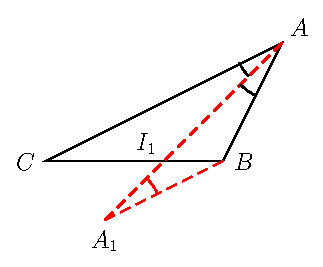
\includegraphics{../images/img005123-1}$$


On a aussi bien sûr les deux autres égalités $I_2=\mbox{bar}\{A(a),C(c)\}$ 
et $I_3=\mbox{bar}\{A(a),B(b)\}$ où $I_2$ et $I_3$ sont les points d'intersection des deux
autres bissectrices avec $(AC)$ et $(AB)$ respectivement.
Soit alors $I'=\mbox{bar}\{A(a),B(b),C(c)\}$. D'après le théorème du barycentre partiel, on a

$$I'=\mbox{bar}\{A(a),I_1(b+c)\}=\mbox{bar}\{B(b),I_2(a+c)\}=\mbox{bar}\{C(c),I_3(a+b)\},$$
ce qui montre que $I'$ est sur $(AI_1)$, $(BI_2)$ et $(CI_3)$, c'est-à-dire sur les trois bissectrices. Par suite,
$I'=I$.}
    \item \question{Déterminer $z$ complexe tel que $O$ soit le centre du cercle inscrit au triangle $(PQR)$ dont les sommets
ont pour affixes respectives $z$, $z^2$ et $z^3$.}
\reponse{Soit $z\in\Cc$.
$$z,\;z^2\;\mbox{et}\;z^3\;\mbox{ne sont pas deux à deux distincts}\Leftrightarrow
z^2=z\;\mbox{ou}\;z^3=z\;\mbox{ou}\;z^3=z^2\Leftrightarrow z\in\{-1,0,1\}.$$
Ensuite, pour $z\notin\{-1,0,1\}$,

$$z,\;z^2\;\mbox{et}\;z^3\;\mbox{sont
alignés}\Leftrightarrow\exists\lambda\in\Rr/\;z^3-z=\lambda(z^2-z)\Leftrightarrow\frac{z^3-z}{z^2-z}\in\Rr\Leftrightarrow z+1\in\Rr\Leftrightarrow z\in\Rr.$$
Finalement, $(z,z^2,z^3)$ est un \og vrai \fg~triangle si et seulement si $z$ n'est pas réel.
Soit alors $z$ un complexe non réel.

\begin{align*}
O\;\mbox{centre du cercle inscrit au triangle}\;(PQR)&\Leftrightarrow O=\mbox{bar}\{P(QR),Q(PR),R(PQ)\}\\
 &\Leftrightarrow z|z^2-z^3|+z^2|z-z^3|+z^3|z-z^2|=0
\Leftrightarrow z.|z|.|1-z|(|z|+z|1+z|+z^2)=0\\
 &\Leftrightarrow|z|+z|1+z|+z^2=0\;(E)\;(\mbox{car}\;z\notin\Rr)
\end{align*}
Ensuite,

\begin{align*}
|z|+z|1+z|+z^2=0&\Leftrightarrow(z+\frac{|z|}{z})+|1+z|=0\Rightarrow z+\frac{|z|}{z}\in\Rr\Leftrightarrow
z+\frac{|z|}{z}={\bar z}+\frac{|z|}{{\bar z}}\\
 &\Leftrightarrow z-{\bar z}-|z|\frac{z-{\bar z}}{z{\bar z}}=0\Leftrightarrow(z-{\bar z})(1-\frac{1}{|z|})=0
\Leftrightarrow1-\frac{1}{|z|}=0\;(\mbox{car}\;z\neq{\bar z})\\
 &\Leftrightarrow|z|= 1
\end{align*}
Posons donc $z=e^{i\theta}$ où $\theta\notin\pi\Zz$. En reportant dans $(E)$, on obtient

\begin{align*}
z\;\mbox{solution de}\;(E)&\Leftrightarrow e^{i\theta}+e^{-i\theta}+|1+e^{i\theta}|=
0\Leftrightarrow2\cos\theta+|e^{i\theta/2}|.|2\cos\frac{\theta}{2}|=0\\
 &\Leftrightarrow\cos\theta+|\cos\frac{\theta}{2}|=0\Leftrightarrow2|\cos\frac{\theta}{2}|^2+|\cos\frac{\theta}{2}|-1=0
\Leftrightarrow|\cos\frac{\theta}{2}|\;\text{est solution de l'équation}\;2X^2+X-1=0\\
 &\Leftrightarrow\left|\cos\frac{\theta}{2}\right|\in\left\{\frac{1}{2},-1\right\}\Leftrightarrow\left|\cos\frac{\theta}{2}\right|=\frac{1}{2}
\Leftrightarrow2\cos^2\frac{\theta}{2}-1=-\frac{1}{2}
\Leftrightarrow\cos\theta=-\frac{1}{2}\Leftrightarrow\theta\in\pm\frac{2\pi}{3}+2\pi\Zz\\
 &\Leftrightarrow
z\in\{j,j^2\}
\end{align*}
Les nombres complexes solutions sont donc $j$ et $j^2$.}
\end{enumerate}
}
